\section{Network Access Layer}

% TODO gigabit, 10gigabit, 40/100gigabit ethernet
% TODO explain CSMA/CD

\subsection{SDU/PDU}

Die Service Data Unit (SDU oder auch Payload) eines Layers ist die Protocol Data
Unit (PDU) des darüberliegenden Layers.

PDU = Protokollinformationen (PCI) + SDU

Layer 1 SDU = Layer 2 PDU


\subsection{Ethernet}
\subsubsection{10Base-T}

\textbf{Wiring}

Transmit (TX) auf Pins 1 und 2\\
Receive (RX) auf Pins 3 und 6

\textbf{Codierung}

Der 10Base-T Standard verwendet Manchester Codierung. Daher ist für 10 Mbit
Datenübertragungsraten eine effektive Übertragungsrate von 20 Mbit erforderlich,
weil für die Codierung eines Bits zwei Signale benötigt werden. Die Bitrate ist
in diesem Fall halb so gross wie die Baudrate.

\textbf{Daten}

Bitdauer:
\[
	\frac{\SI{1}{\second}}{\SI{e7}{\bit}} = \SI{100}{\ns}
\]

Ausbreitung Elektromagnetischer Wellen im Kabel: 
\[
	\frac{2}{3} \cdot 300\cdot \SI{e6}{\meter\per\second} = \SI{0.2}{\meter\per\ns}
\]

Länge eines Bits im Kabel:
\[
	\SI{100}{\ns} \cdot \SI{0.2}{\meter\per\ns} = \SI{20}{\meter}
\]


\subsubsection{100Base-TX}

\textbf{Wiring}

Transmit (TX) auf Pins 1 und 2\\
Receive (RX) auf Pins 3 und 6

\textbf{Codierung}

Der 100Base-TX Standard verwendet eines sogenanntes 4B5B Encoding
(Block-Codierung). Jedes 4 Bit Wort wird auf ein 5 Bit Wort abgebildet, so dass
nie mehr als 3 aufeinander folgende Nullen vorhanden sind. Somit ist eine
sogenannte Symbolrate/Baudrate von +25\%, also 125 Mbps, notwendig.

Um das Übertragene Spektrum zu verkleinern, werden die Bits zusätzlich mittels
MLT-3 (Multi-Level-Transition) Verfahren codiert.

Die Taktrückgewinnung mit reiner MLT-3 Codierung ist nicht möglich, durch die
vorangegangene 4B5B Codierung jedoch schon. Zusätzlich bleiben durch die 4B5B
Codierung weitere $2^5-2^4=16$ Codes übrig, die zur
Synchronisation/Signalisierung verwendet werden können.

\textbf{Daten}

Bitdauer:
\[
	\frac{\SI{1}{\second}}{\SI{e8}{\bit}} = \SI{10}{\ns}
\]

Länge eines Bit im Kabel:
\[
	\SI{10}{\ns} \cdot \SI{0.2}{\meter\per\ns} = \SI{2}{\meter}
\]


\subsection{ADSL}

ADSL läuft auf über die reguläre Telefon-Kupferleitung. Daher kann das
Frequenzband von 0~kHz bis 30~kHz nicht genutzt werden, da dieses durch das
Analog-Telefon bereits belegt ist.


\subsubsection{MAC-Frame}

Die Minimallänge eines MAC Frames beträgt 64 Bytes, bedingt durch den CSMA/CD
Mechanismus zur Kollisionsdetektion.

Die Maximalgrösse beträgt 1500 Bytes Payload + 12 Bytes SA/DA + 2 Bytes LEN/PT +
4 Bytes Checksum = 1518 Bytes an Daten. Hinzu kommen noch 8 Bytes für Preamble
und SFD.


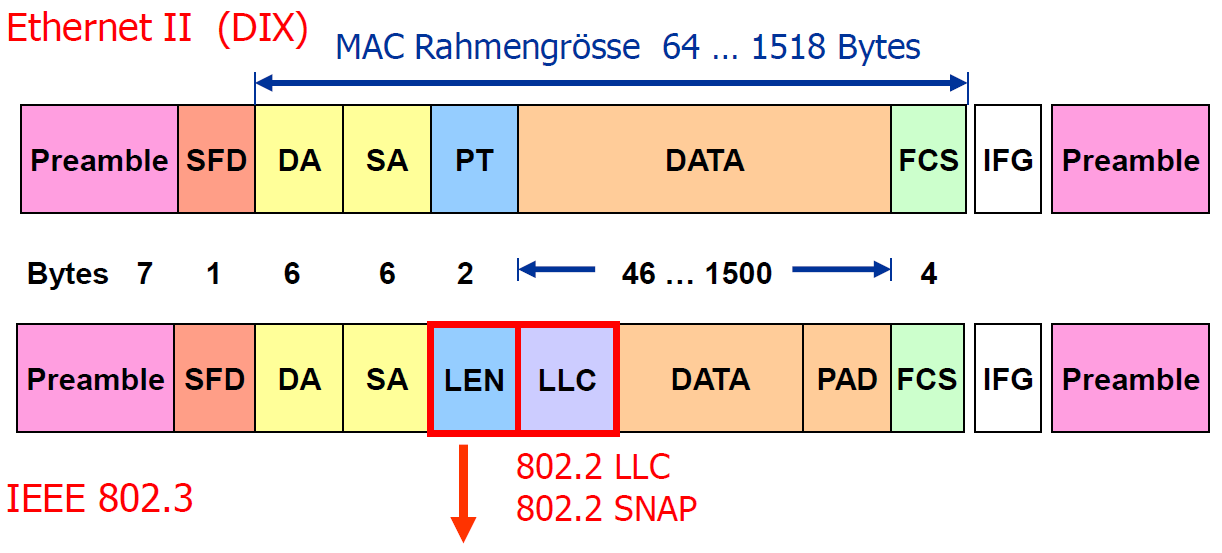
\includegraphics[scale=0.5]{media/MACFrame.png}

\textbf{Ethernet II}

Ethernet II (DIX) Pakete werden durch einen PT grösser als 1500
(0x05DC) gekennzeichnet. Payloadtype für IP: 0x800, für ARP: 0x806.

\textbf{802.3}

Ethernet 802.3 Pakete sind durch Angaben im LEN Feld kleiner als 1500
gekennzeichnet. Die Länge gibt die PDU Länge des LLC Protokolls an.


\subsubsection{Kollisionen}

Kollisionen könnnen nur in Half-Duplex-Mode Übertragungen auftreten. Im
Full-Duplex-Mode werden zwei separate Adernpaare zum Senden und Empfangen der
Daten verwendet, Kollisionen können so physikalisch nicht auftreten.


\subsection{WLAN}

\subsubsection{Amplitudenmodulation}

% TODO unmatched parentheses, add explanations
\[
	\cos (2\pi \cdot F_N) \cdot \cos (2\pi \cdot F_T)
	= \frac{1}{2}(\cos (2\pi \cdot F_T - 2\pi \cdot F_N)
	+ cos(2\pi \cdot F_T + 2\pi \cdot F_N)
\]

Somit hat sich zum einen die Regellage verschoben und es ist noch eine Kehrlage
hinzugekommen: $\cos (2\pi F_T - F_N)$.


\subsection{MAC-Adressen}

Das LSB im ersten Adddress Byte (Most Significant Octet) der Destination Address
ist das Individual/Group Bit.

\begin{tabular}[h]{|l|l|}
	\hline
  \textbf{Value} & \textbf{Address Type} \\
	\hline
  0 & Individual Address \\
  1 & Multicast/Broadcast Address \\
	\hline
\end{tabular}

Das zweite Bit ist das Universal/Local Bit.

\begin{tabular}[h]{|l|l|}
	\hline
  \textbf{Value} & \textbf{Address Type} \\
	\hline
  0 & Globally Administered Address \\
  1 & Locally Administered Address \\
	\hline
\end{tabular}
